%\documentclass[10pt,a4paper]{article}
\documentclass[12pt,a4paper]{article}
\usepackage{graphicx,amsmath}
%\usepackage{subfigure}
\usepackage{float}
\usepackage[german]{babel}
\usepackage[utf8]{inputenc}
\setcounter{secnumdepth}{4}
\usepackage[top=2cm, bottom=2.5cm, left=3cm, right=3cm]{geometry}
\begin{document}


%\title{Bachelorarbeit}
%\author{Richard Kullmann}
%\date{02.06.2017}

\thispagestyle{empty}
%\setcounter{page}{2}
\newpage
\tableofcontents
\thispagestyle{empty}
\newpage
\pagenumbering{arabic}
\section{Phasenportraits}
Um die Dynamik im Phasenraum noch einmal besser zu veranschaulichen, habe ich kurze Trajektorien von verschiedenen Startpunkten im deterministischen Modell betrachtet. Da mit bloßem Auge kaum Unterschiede zwischen den Phasenraumportraits bei verschiedenen Strömen $I$ auszumachen sind, habe ich noch die Isoklinen (Nullclines) geplottet: \begin{figure}[H]
	\centering
	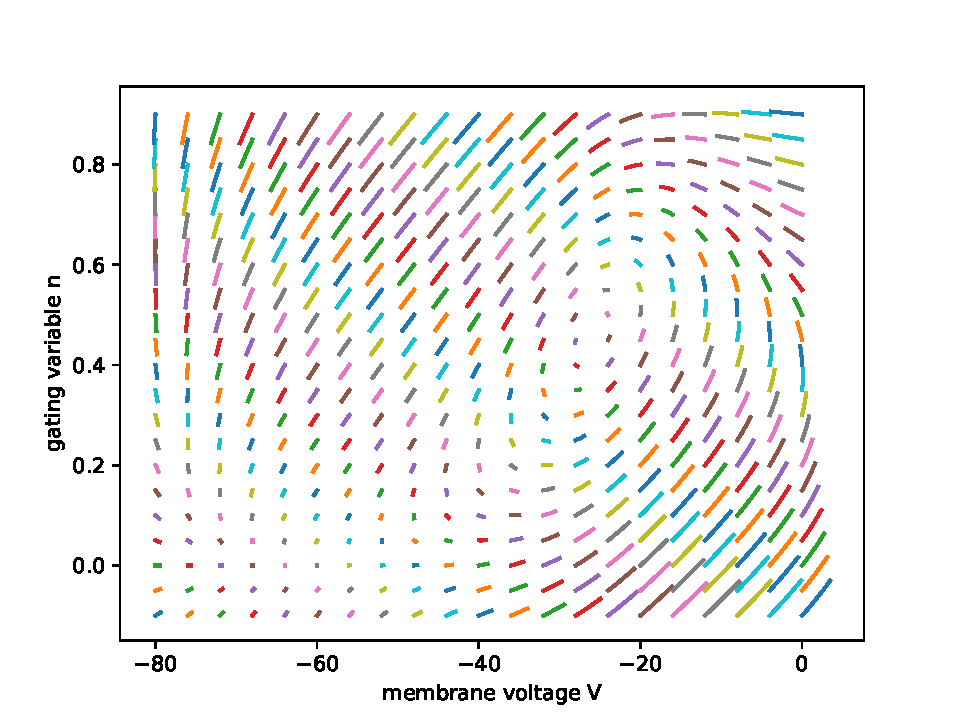
\includegraphics[scale=0.9]{phaselinessh6.pdf} 
	\caption{kurze Phasenraumtrajektorien bei $I=6$}
	\label{prs}
\end{figure}  
\begin{figure}[H]
	\centering
	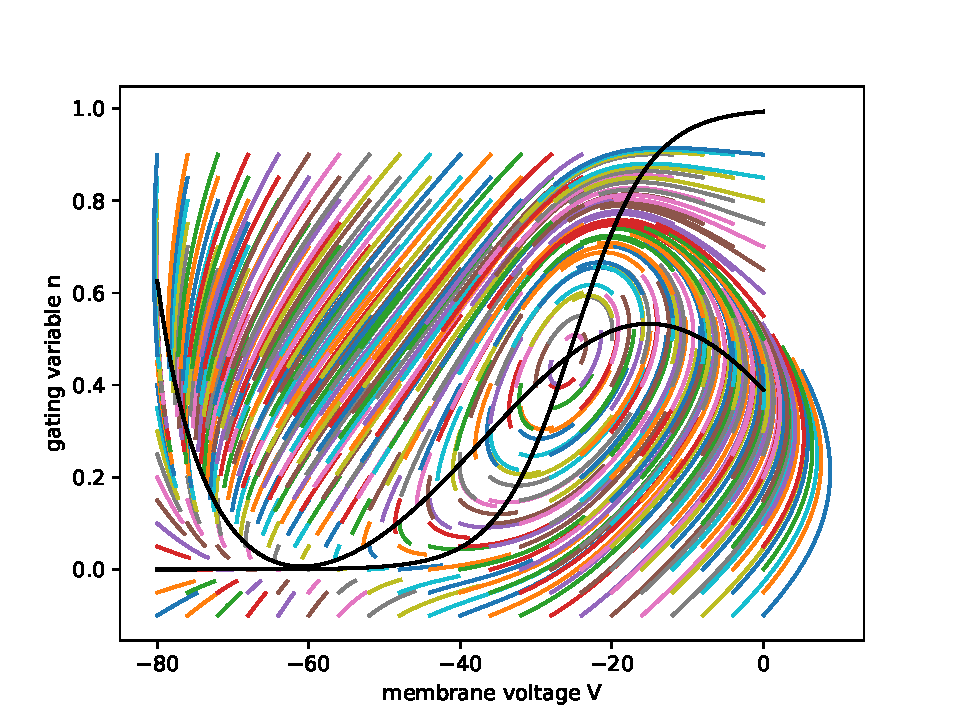
\includegraphics[scale=0.9]{phaseliness6wn.pdf} 
	\caption{lange Phasenraumtrajektorien bei $I=6$ mit Isoklinen in schwarz}
	\label{prll}
\end{figure} 
\begin{figure}[H]
	\centering
	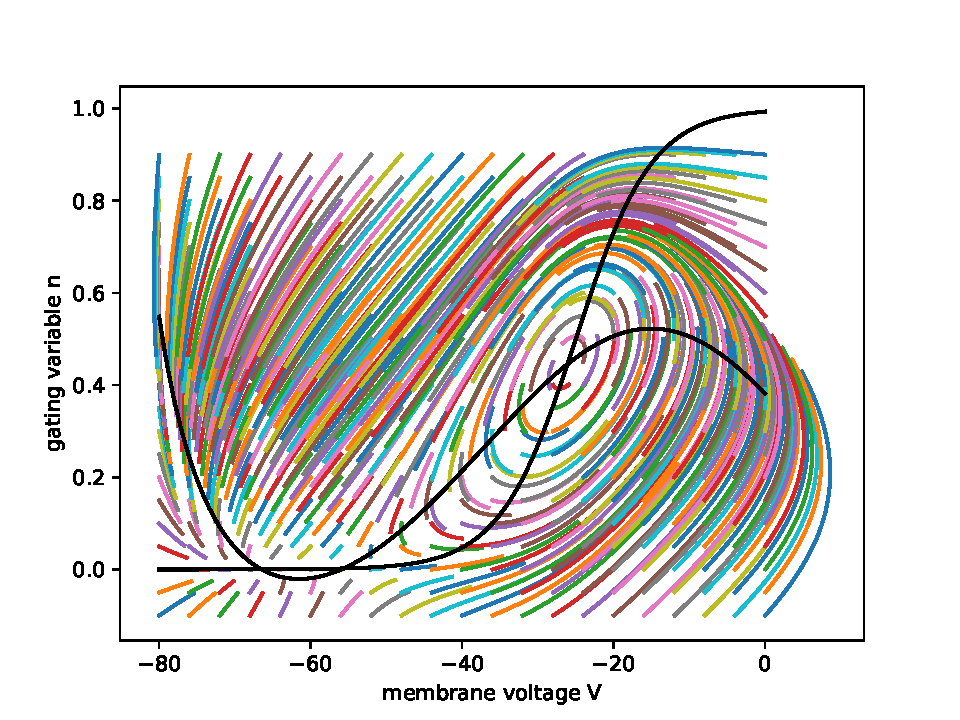
\includegraphics[scale=0.9]{phaseliness-1wn.pdf} 
	\caption{lange Phasenraumtrajektorien bei $I=-1$ mit Isoklinen in schwarz}
	\label{prls}
\end{figure} 
Man kann klar erkennen, wie bei $I=6$ die beiden Gleichgewichtspunkte ineinander übergelaufen sind. Zudem ergibt sich im Zentrum des Grenzzyklus der instabile Gleichgewichtspunkt beim Schnittpunkt der Isoklinen.
\section{Fano-Faktor im Neuronenmodell}
Wie angekündigt, wurde der Fano-Faktor nun noch einmal mit mehr Durchläufen (entspricht einer höheren Anzahl von Neuronen) wiederholt, mit einer Rechendauer von 20h pro Punkt. Dabei hat sich überraschenderweise herausgestellt, dass der Diffusionskoeffizient - und dementsprechend auch der Fano-Faktor - ein Maximum bei einer Rauschintensität größer als 0 erreicht, hier bei etwa $D=3$, entgegen den Erwartungen aus dem mechanischen Modell. Das Phänomen der 'Giant Diffusion' scheint hier also doch nicht aufzutreten.
\begin{figure}[H]
	\centering
	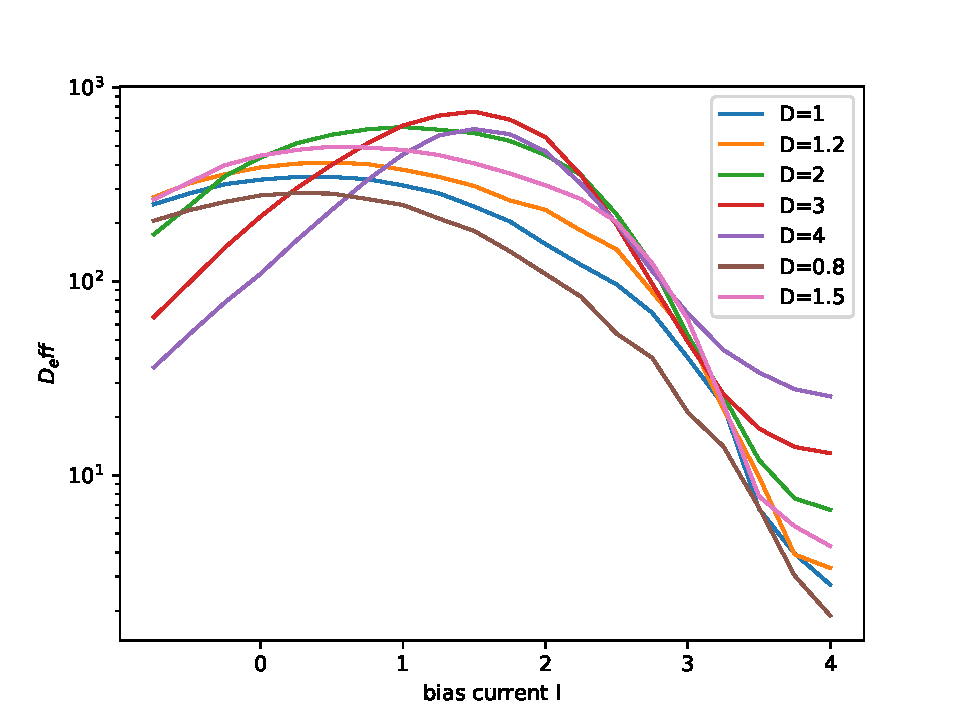
\includegraphics[scale=0.9]{dneurpm.pdf} 
	\caption{Diffusionskoeffizienten für verschiedene Rauschintensitäten}
	\label{dnp}
\end{figure} 
\begin{figure}[H]
	\centering
	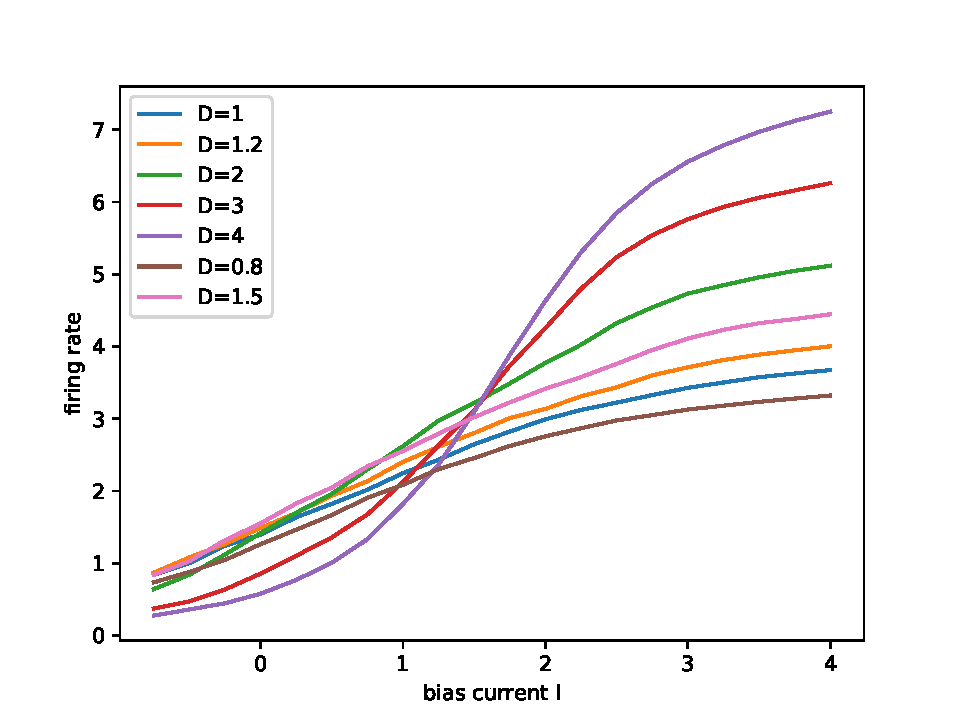
\includegraphics[scale=0.9]{gneurpm.pdf} 
	\caption{Feuerraten für verschiedene Rauschintensitäten}
	\label{gnp}
\end{figure} 
\begin{figure}[H]
	\centering
	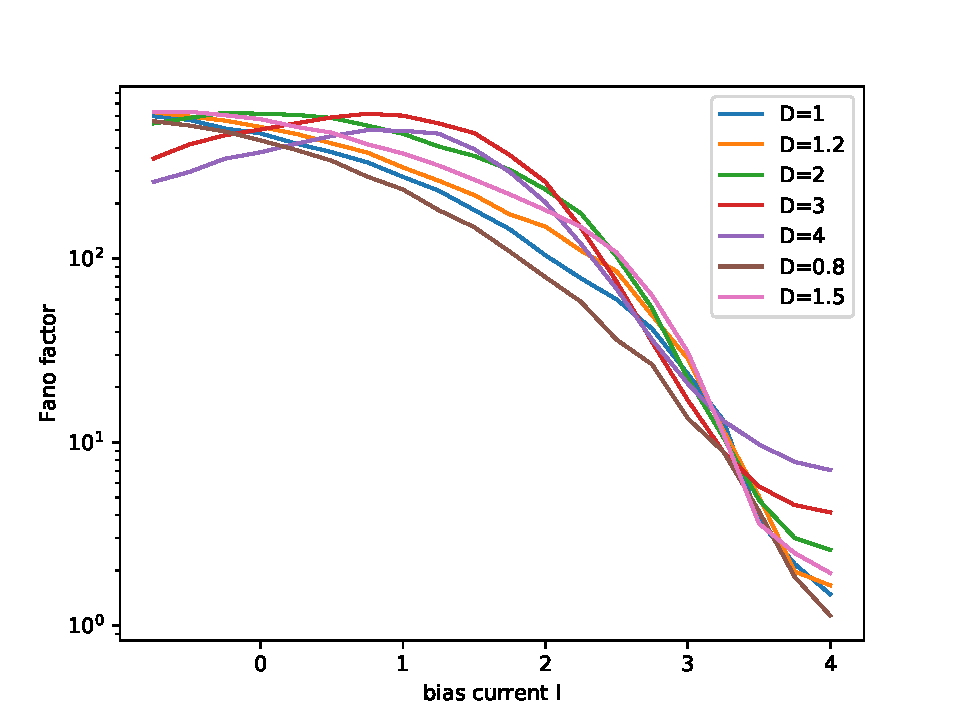
\includegraphics[scale=0.9]{fneurpm.pdf} 
	\caption{Fano-Faktoren für verschiedene Rauschintensitäten}
	\label{fnp}
\end{figure} 
Beim Betrachten der Feuerraten fällt auf, dass für $D=2,3,4$ ein klarer Schnittpunkt zu erkennen ist, während sich die anderen Kurven dann immer weiter von diesem entfernen. Für $I>=2$ verhalten sich die Feuerraten jedoch erwartungsgemäß, also proportional zur Rauschintensität. Kann es sein, dass es eine andere Kombination von Parametern gibt, die Giant Diffusion aufweist, auch wenn sie in diesem Fall nicht auftritt?\\
Weiteres Vorgehen: Finden der Rauschintensität, für die der Diffusionskoeffizient sein Maximum erreicht. 
\section{mechanisches Modell}
Die Rechnungen für das mechanische Modell wurden vorerst fertig gestellt: 
\begin{figure}[H]
	\centering
	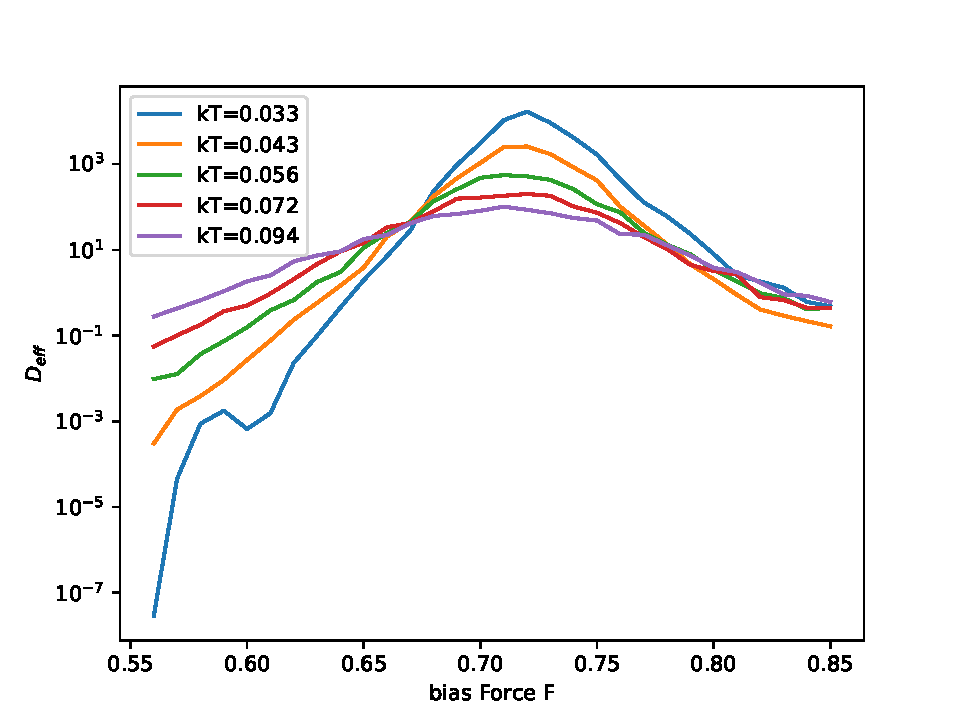
\includegraphics[scale=0.9]{mechdsht.pdf} 
	\caption{Diffusionskoeffizienten für verschiedene Rauschintensitäten}
	\label{mdsh}
\end{figure}
\begin{figure}[H]
	\centering
	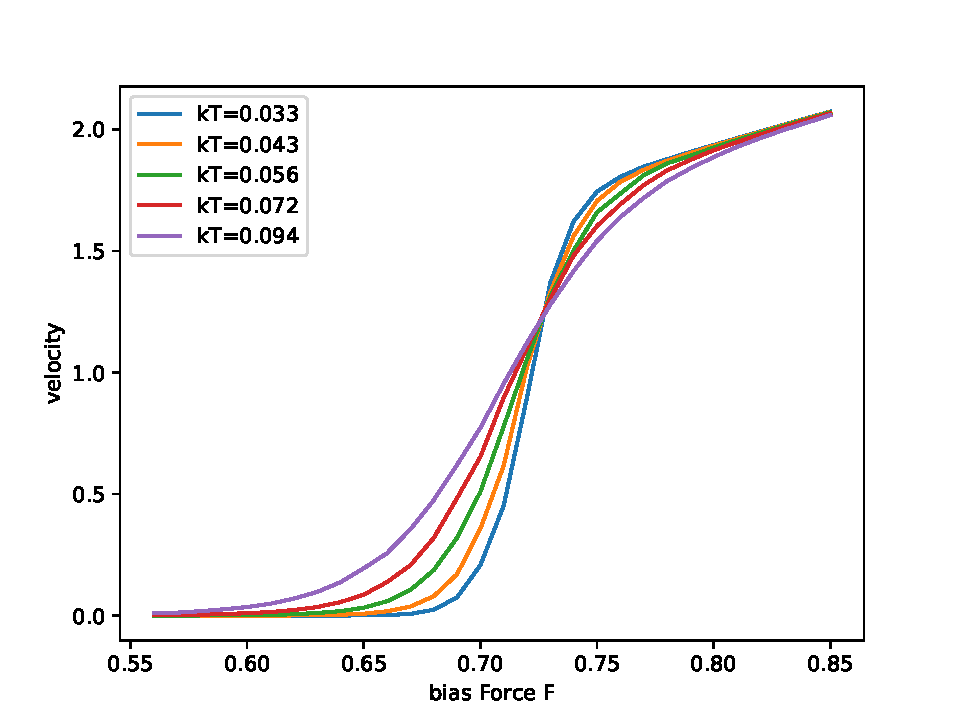
\includegraphics[scale=0.9]{mechgsht.pdf} 
	\caption{mittlere Geschwindigkeiten für verschiedene Rauschintensitäten}
	\label{mgsh}
\end{figure}
\begin{figure}[H]
	\centering
	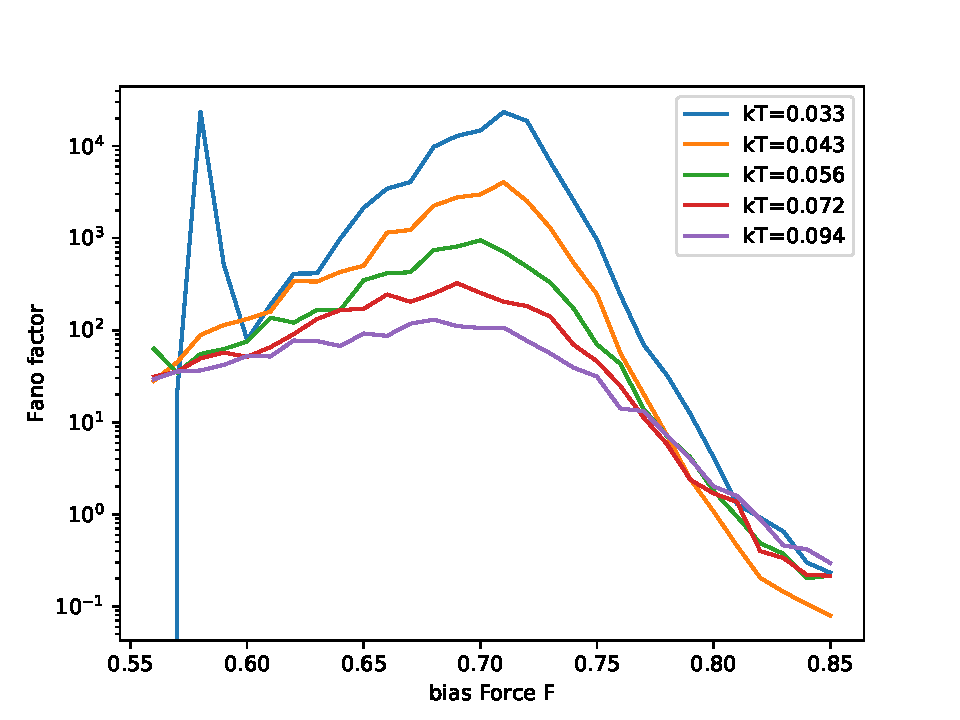
\includegraphics[scale=0.9]{mechfsht.pdf} 
	\caption{Fano-Faktoren für verschiedene Rauschintensitäten}
	\label{mfsh}
\end{figure}
Die extremen Schwankungen für den Fano-Faktor resultieren aus der niedrigen Geschwindigkeit, die nahe bei 0 auch negative Werte erreichen kann.\\
Es stellt sich heraus, dass auch mehrmaliges Wiederholen der Simulation für $kT=0.033$ nicht den gewünschten Schnittpunkt bei $F\approx 0.78$ ergibt; der linke Schnittpunkt kann jedoch sehr gut reproduziert werden.\\
Weiteres Vorgehen: Ausführliche Untersuchung des Verhaltens des Diffusionskoeffizienten für verschiedene Laufzeiten, dann
Wiederholen der Rechnungen mit höherer Genauigkeit.
\end{document}

